\documentclass[12pt]{article}
\usepackage[utf8]{inputenc}
\usepackage[T1]{fontenc}
\usepackage[polish]{babel}
\usepackage{geometry}
\usepackage{tabularx}
\usepackage[table,xcdraw,dvipsnames]{xcolor}
\usepackage{color}
\usepackage{subfig}
\usepackage{sidecap}
\usepackage{wrapfig}
\usepackage{float}
\usepackage{enumerate}
\usepackage{graphicx}
\usepackage{multirow}
\usepackage{hyperref}
\usepackage{titlesec}
\usepackage{amsmath}
\usepackage{anyfontsize}
\usepackage{indentfirst}
\usepackage{listings}
\usepackage{multicol}
\usepackage{pgfplots}
\usepackage{fancyhdr}

\newgeometry{tmargin=1.8cm,bmargin=1.8cm,lmargin =1.8cm,rmargin=1.8cm}

\begin{document}
\renewcommand{\figurename}{Rys.}

% \newcommand{\zdjecie}[4]
% {
%     \begin{figure}[H]
%         \renewcommand{\figurename}{Rys.}
%         \centering
%         \includegraphics[]{#2}
%         \caption{#3}
%         \label{#4}
%     \end{figure}
% }

\begin{titlepage}
\begin{figure}
    \centering
    
\includegraphics[width=18cm]{logo-PWr.png}
    \label{fig:pwr}
\end{figure}
    \begin{center}
        \LARGE \textbf{ Wydział Elektroniki, Fotoniki i Mikrosystemów }\\ 
        \vspace{70pt}
        \Huge \textit{ Sterowanie Procesami Ciągłymi}  \\
    \end{center}
    \vspace{30pt}
    \hrule
    \vspace{1pt}
    \hrule
    \begin{center}
        {\fontsize{30}{50}\selectfont Sprawozdanie nr 1\\ }
        \vspace{10pt}
        {\fontsize{25}{25}\selectfont Charakterystyki czasowe  }
    \end{center}
    \hrule
    \vspace{1pt}
    \hrule
    \begin{flushright}
        \vspace{50pt}

        \textit{\Large Prowadzący:}\\
        \Large dr hab. inż. Grzegorz Mzyk\\
        \vspace{10pt}
        \textit{\Large Wykonała:}\\
        \Large Zuzanna Mejer, 259382 \\
        \vspace{10pt}
        \textit{\Large Termin zajęć:}\\
        \Large czwartek TP, 9:15\\
        \vspace{10pt}
    
    \end{flushright}
    \vspace{60pt}
    \begin{center}
        \large Wrocław, \today r.
    \end{center}
\end{titlepage}
    
    
\tableofcontents
\newpage

\section{Cel ćwiczenia}
Celem ćwiczenia była identyfikacja obiektu dyskretnego na podstawie wygenerowanych danych oraz późniejsza ocena jakości identyfikacji w zależności od liczby pomiarów.

\section{Generowanie danych}
Dany jest obiekt dyskretny opisany wzorem:
\begin{equation}
    y_k = 3u_k+2u_{k-1} + 1u_{k-2} + z_k,
    \label{wzor_dyskretny}
\end{equation}
gdzie $z_k, u_k$ są od siebie niezależne. Wejście $u_k$ jest opisane funkcją \textit{randn}, która generuje liczby o rozkładzie normalnym. Z kolei $z_k$ jest opisane funkcją \textit{rand - 0,5}, która generuje liczby o rozkładzie równomiernym z zakresu [-0,5 ; 0,5]. Wykorzystując przedstawiony skrypt (rys. \ref{generowanie_danych_skrypt}), wygenerowano ciąg par (rys. \ref{generowanie_danych_dane}):
\begin{equation}
    \{(u_k, y_k)\}^N_{k=3}
\end{equation}
gdzie $N$ to liczba ciągu par. Rozpoczęto od $k=3$ ze względu na nieznajomość wcześniejszych zdarzeń $(u_0, u_{-1})$.

\begin{figure}[H]
    \centering
    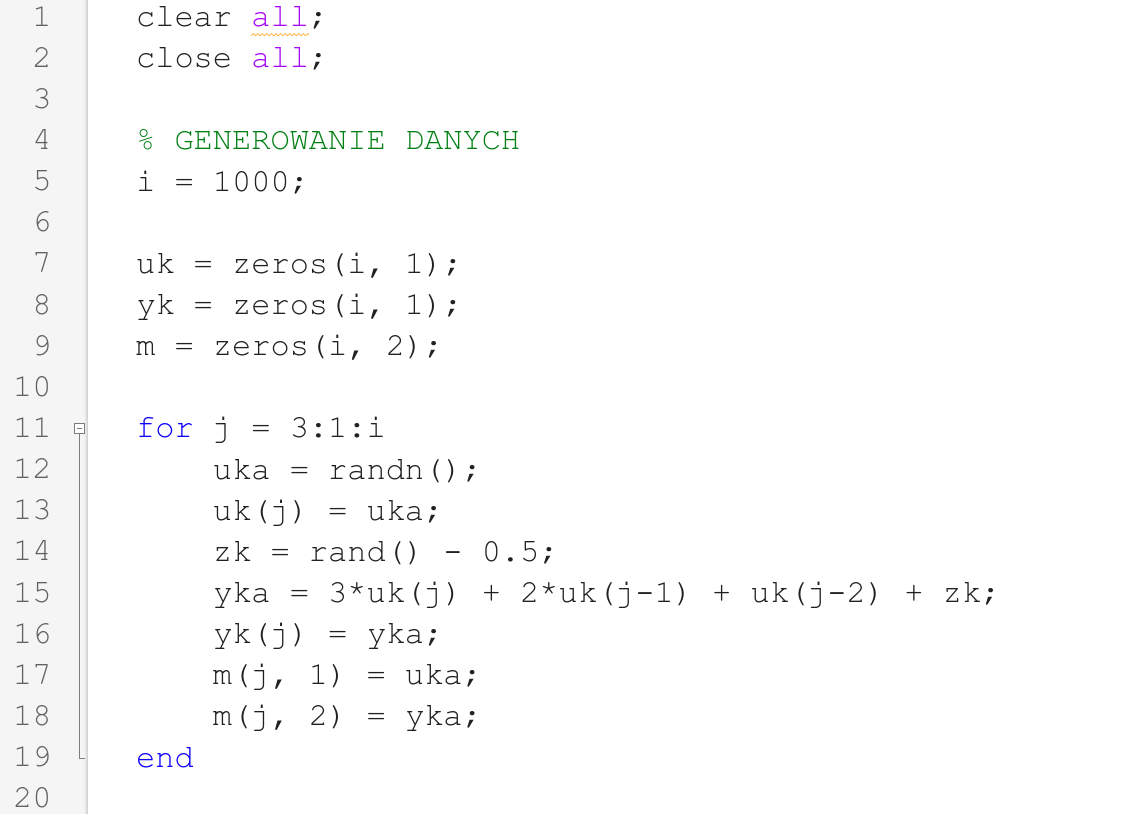
\includegraphics[scale=0.4]{generowanie_danych_skrypt.png}
    \caption{Skrypt w Matlabie do wygenerowania danych}
    \label{generowanie_danych_skrypt}
\end{figure}

\begin{figure}[H]
    \centering
    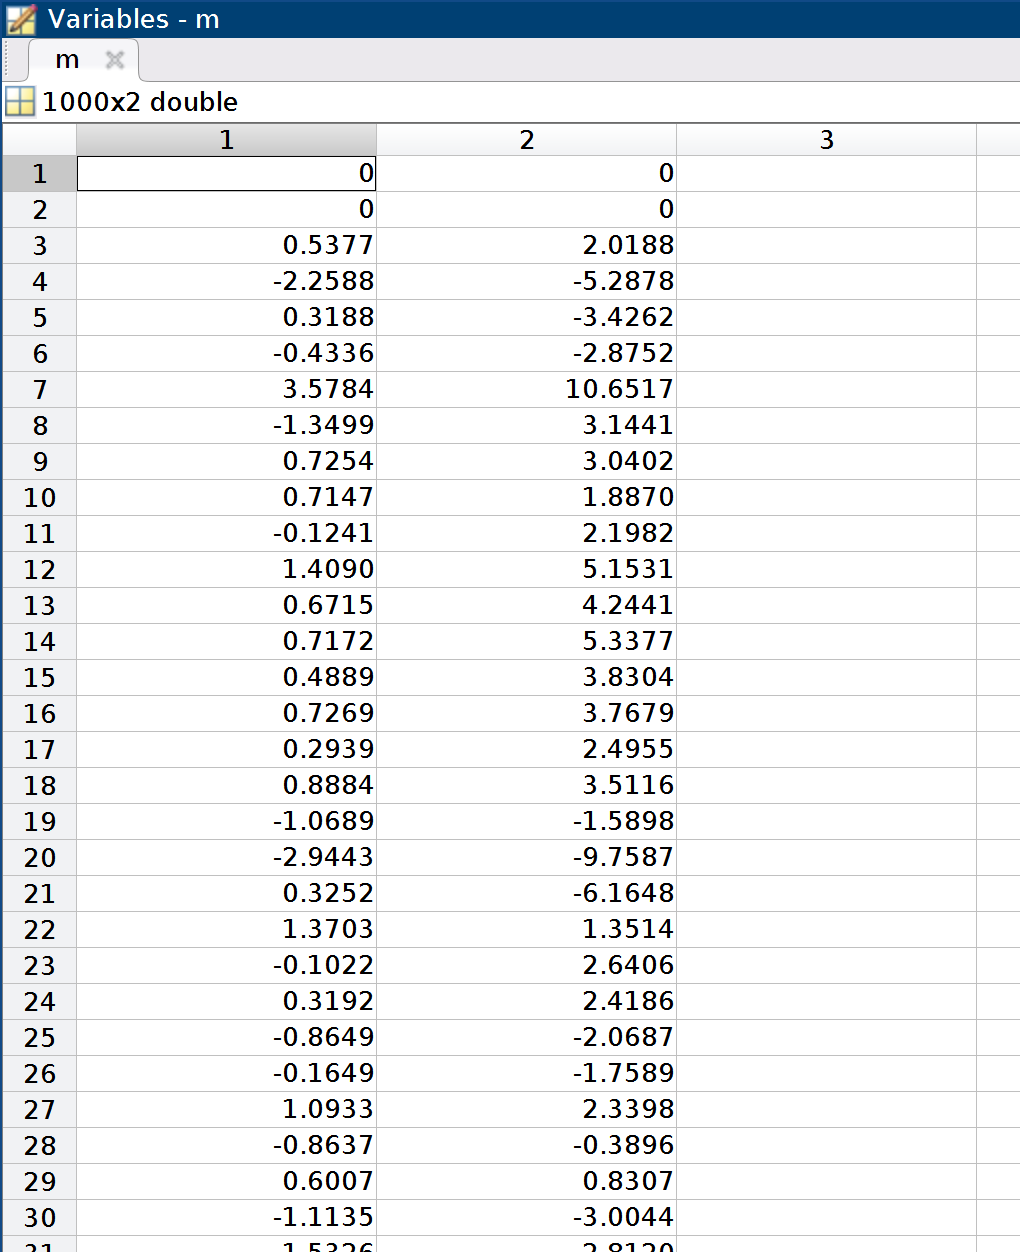
\includegraphics[scale=0.3]{generowanie_danych_dane.png}
    \caption{Fragment wygenerowanego ciągu 1000 par od trzeciego elementu}
    \label{generowanie_danych_dane}
\end{figure}


\section{Identyfikacja obiektu}
W tej części zakłada się, że nie jest znany dokładny dyskretny opis obiektu (\ref{wzor_dyskretny}), a jedynie jego postać:
\begin{equation}
    y_k = a_0 \cdot u_k+a_1 \cdot u_{k-1} + a_2 \cdot u_{k-2} + z_k,
\end{equation}
gdzie $a_0, a_1, a_2$ to wartości szukane. W celu zidentyfikowania obiektu wygenerowano macierze $X_N$ oraz $Y_N$ zawierające kolejne elementy ciągu par:
\begin{equation}
    X_N = \begin{bmatrix}
        u_3 & u_2 & u_1\\
        u_4 & u_3 & u_2\\
        ... & ... & ... \\
        u_N & u_{N-1} & u_{N-2}
        \end{bmatrix}
    \hspace{30pt}
    Y_N = \begin{bmatrix}
        y_1\\
        y_2\\
        ...\\
        y_N
    \end{bmatrix}
\end{equation}
Ze względu na nieznajomość wcześniejszych zdarzeń ($u_0$, $u_{-1}$), wycięto 2 pierwsze wiersze macierzy $X_N$, których nie pokazano już w powyższym wzorze.

Do znalezienia $a_0, a_1, a_2$ przyjęto estymator:

\begin{equation}
    \hat{\varTheta} = \begin{bmatrix}
        \hat{a_0}\\
        \hat{a_1}\\
        \hat{a_2}
    \end{bmatrix} 
    = {(X_N^T \cdot X_N)}^{-1} \cdot X_N^T \cdot Y_N
\end{equation}
W celu wyznaczenia estymatora wygenerowano skrypt w Matlabie (rys. \ref{identyfikacja_skrypt}). Otrzymane wyniki zostały przedstawione na rys. \ref{identyfikacja_estymator}


\begin{figure}[H]
    \centering
    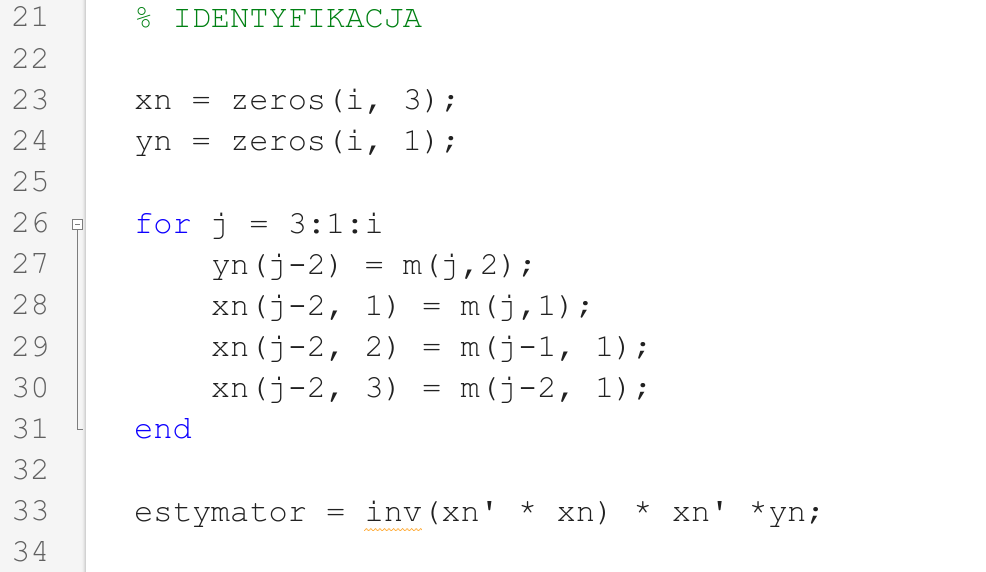
\includegraphics[scale=0.4]{identyfikacja_skrypt.png}
    \caption{Skrypt w Matlabie do wyznaczenia wartości estymowanych}
    \label{identyfikacja_skrypt}
\end{figure}

\begin{figure}[H]
    \centering
    \subfloat{
        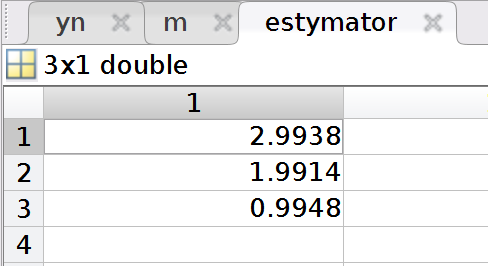
\includegraphics[scale=0.3]{identyfikacja1.png}
    }
    \quad
    \subfloat{
        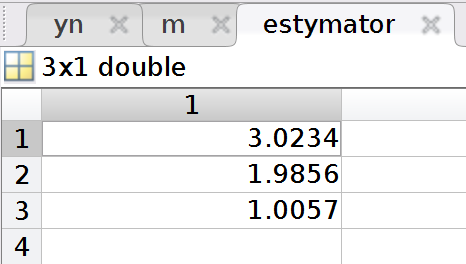
\includegraphics[scale=0.3]{identyfikacja2.png}
    }
    \subfloat{
        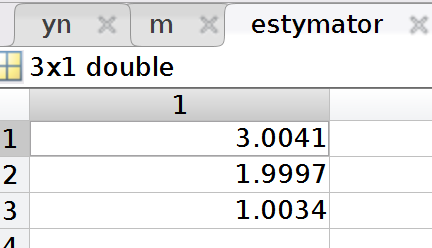
\includegraphics[scale=0.3]{identyfikacja3.png}
    }
    
    \caption{Oszacowany estymator wartości $a_0, a_1, a_2$ - 3 próby}
    \label{identyfikacja_estymator}
\end{figure}
Na rys. \ref{identyfikacja_estymator} przedstawione zostały 3 próby wyliczenia estymatora. Przyjął on wartości:
\begin{equation}
    \hat{\varTheta}_1 \approx \begin{bmatrix}
        2,99\\
        1,99\\
        0,99
    \end{bmatrix} 
    \hspace{30pt}
    \hat{\varTheta}_2 \approx \begin{bmatrix}
        3,02\\
        1,99\\
        1,01
    \end{bmatrix} 
    \hspace{30pt}
    \hat{\varTheta}_3 \approx \begin{bmatrix}
        3,00\\
        2,00\\
        1,00
    \end{bmatrix} 
\end{equation}
Zatem w przybliżeniu: $a_0 = 3$, $a_1=2$, $a_2=1$, co zgadza się z rzeczywistym opisem obiektu dyskretnego (\ref{wzor_dyskretny}).

\section{Błąd estymatora i wielokrotne powtórzenie pomiaru}
Wyznaczono błąd, odejmując wartość rzeczywistą od wartości pochodzącej z identyfikacji, a następnie wyznaczono normę euklidesową otrzymanego wektora:
\begin{equation}
    \Delta_N = norm(\hat{\varTheta} - \varTheta)
\end{equation}
Skrypt opisany w poprzednich punktach (rys. \ref{generowanie_danych_skrypt} \ref{identyfikacja_skrypt}) powtórzono $R$ razy po to, żeby otrzymać wiele estymatorów i żeby móc obliczyć uśredniony błąd estymatora dla danej liczby próbek N:
\begin{equation}
    E(N) = \frac{1}{R} \sum_{R = 1}^{R} \Delta_N  
\end{equation}
Ponadto, całość powtórzono jeszcze kilkukrotnie dla różnej liczby próbek $N = 100 : 500 : 10 000$ (rys. \ref{caly_skrypt1}, \ref{caly_skrypt2}).

\begin{figure}[H]
    \centering
    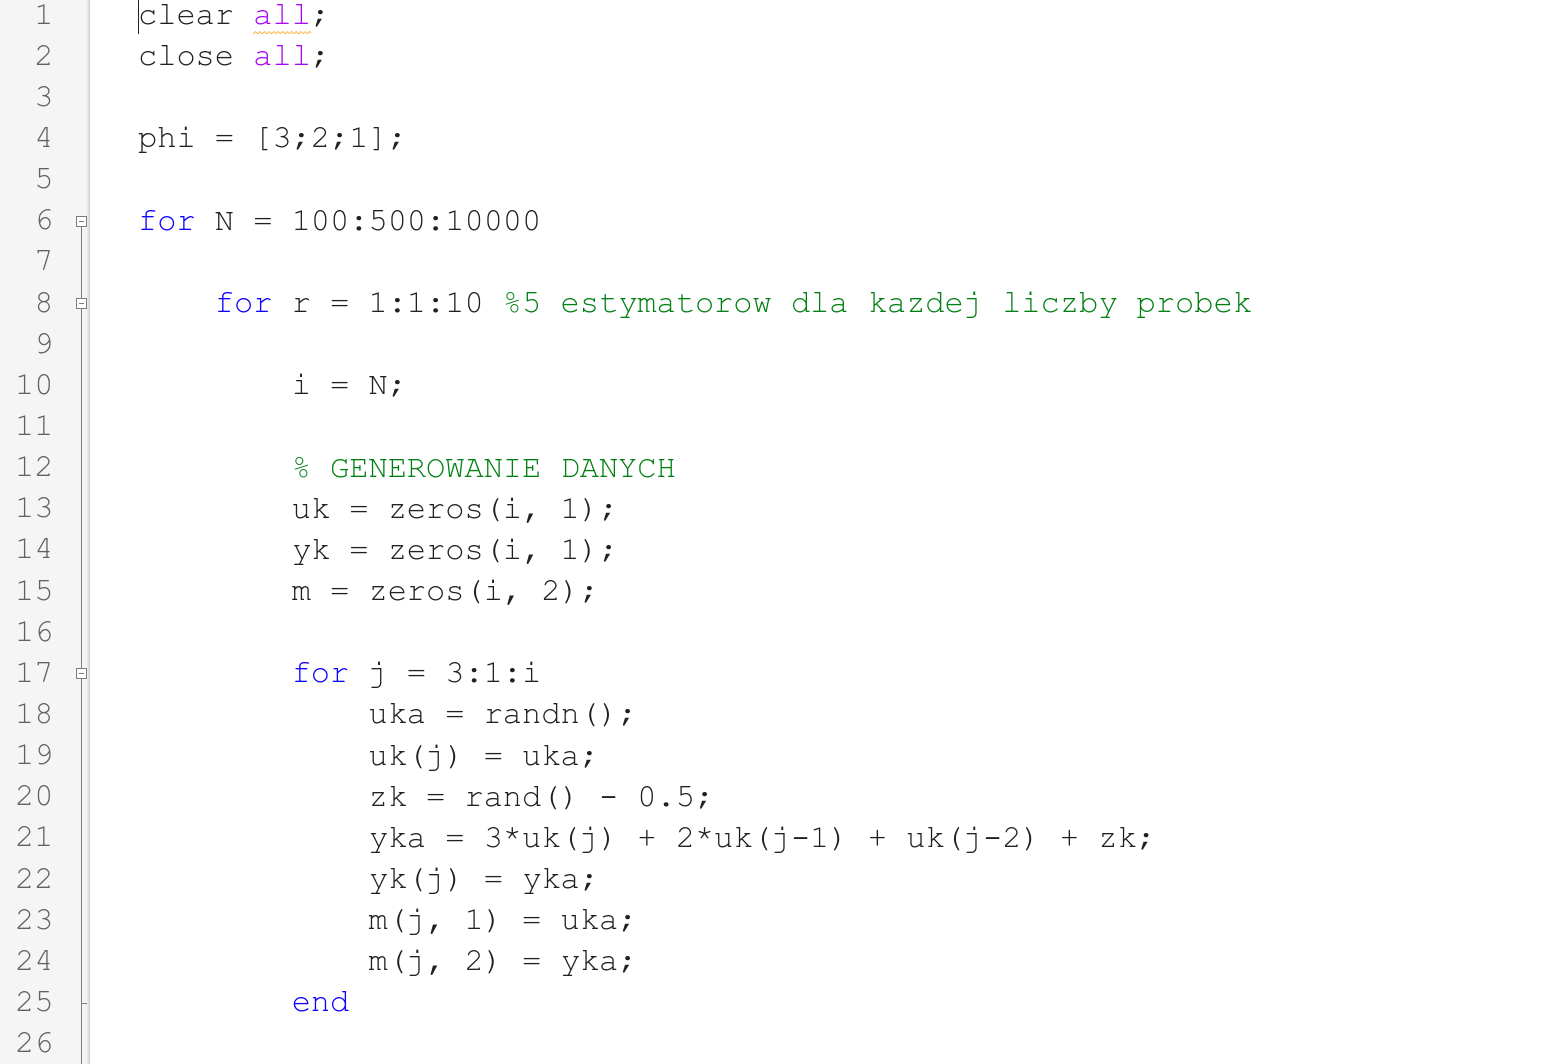
\includegraphics[width = \textwidth]{caly_skrypt1.png}
    \caption{Cały skrypt do wyznaczenia zależności błędu od liczby pomiarów}
    \label{caly_skrypt1}
\end{figure}

\begin{figure}[H]
    \centering
    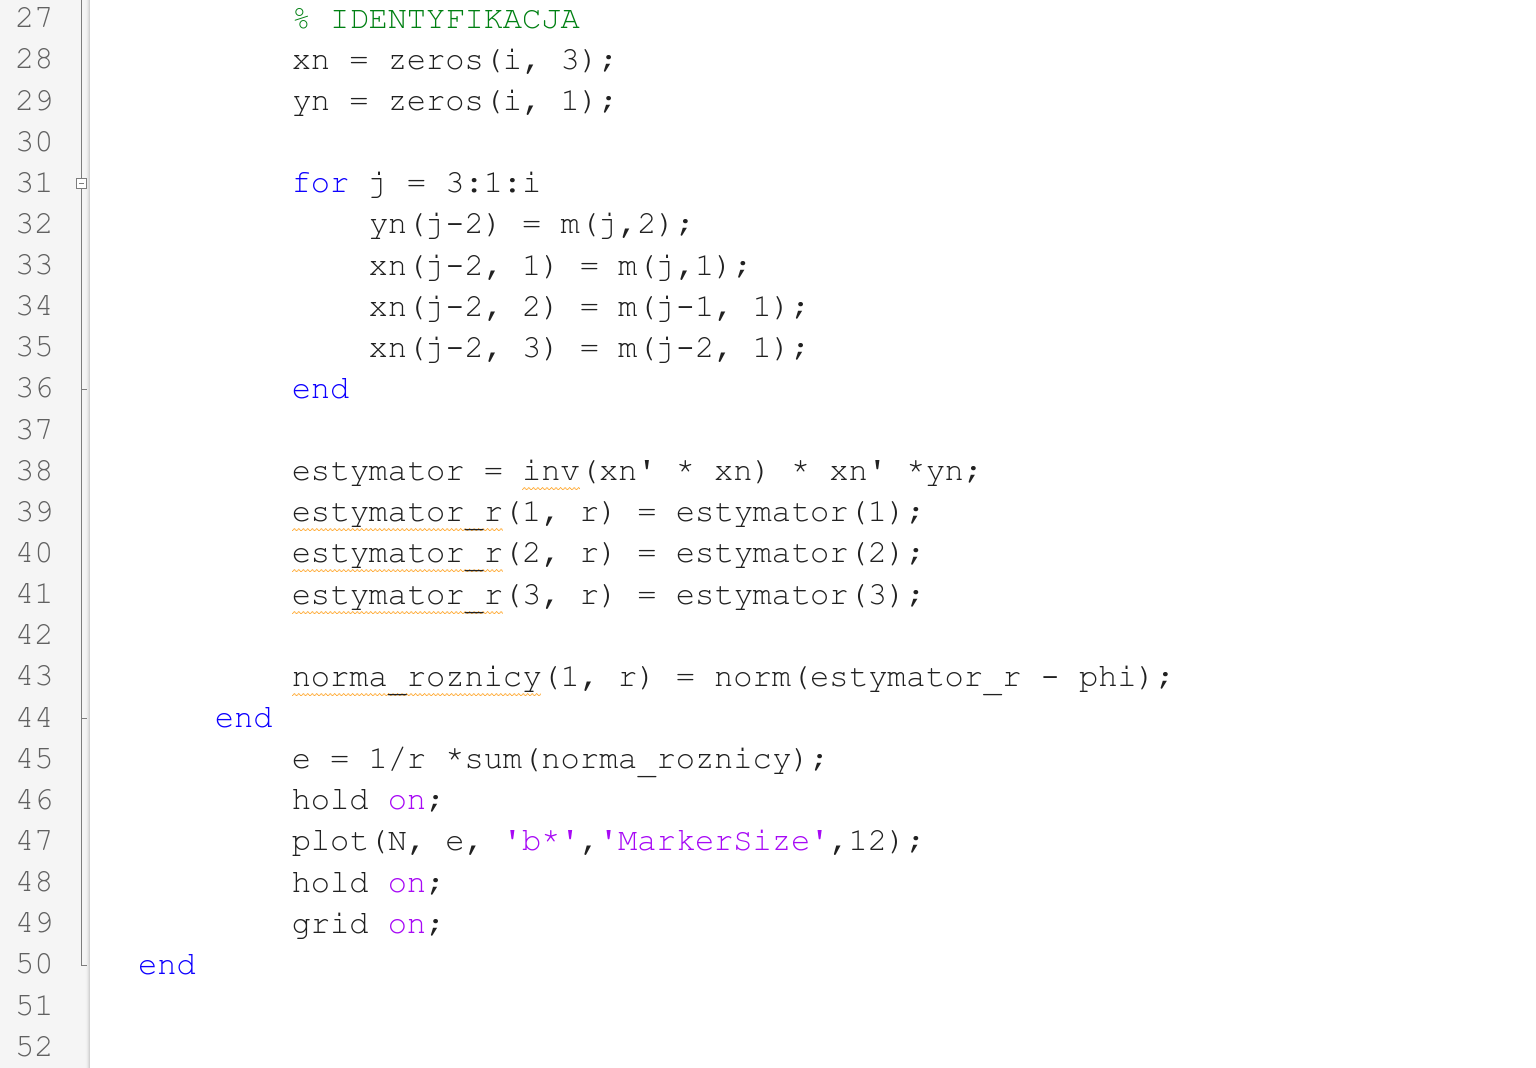
\includegraphics[width = \textwidth]{caly_skrypt2.png}
    \caption{Cały skrypt do wyznaczenia zależności błędu od liczby pomiarów - kontynuacja}
    \label{caly_skrypt2}
\end{figure}



Dzięki temu narysowano jaki jest wpływ liczby pomiarów na średni błąd estymatora (rys. \ref{blad_pomiaru1}, \ref{blad_pomiaru2}).

\begin{figure}[H]
    \centering
    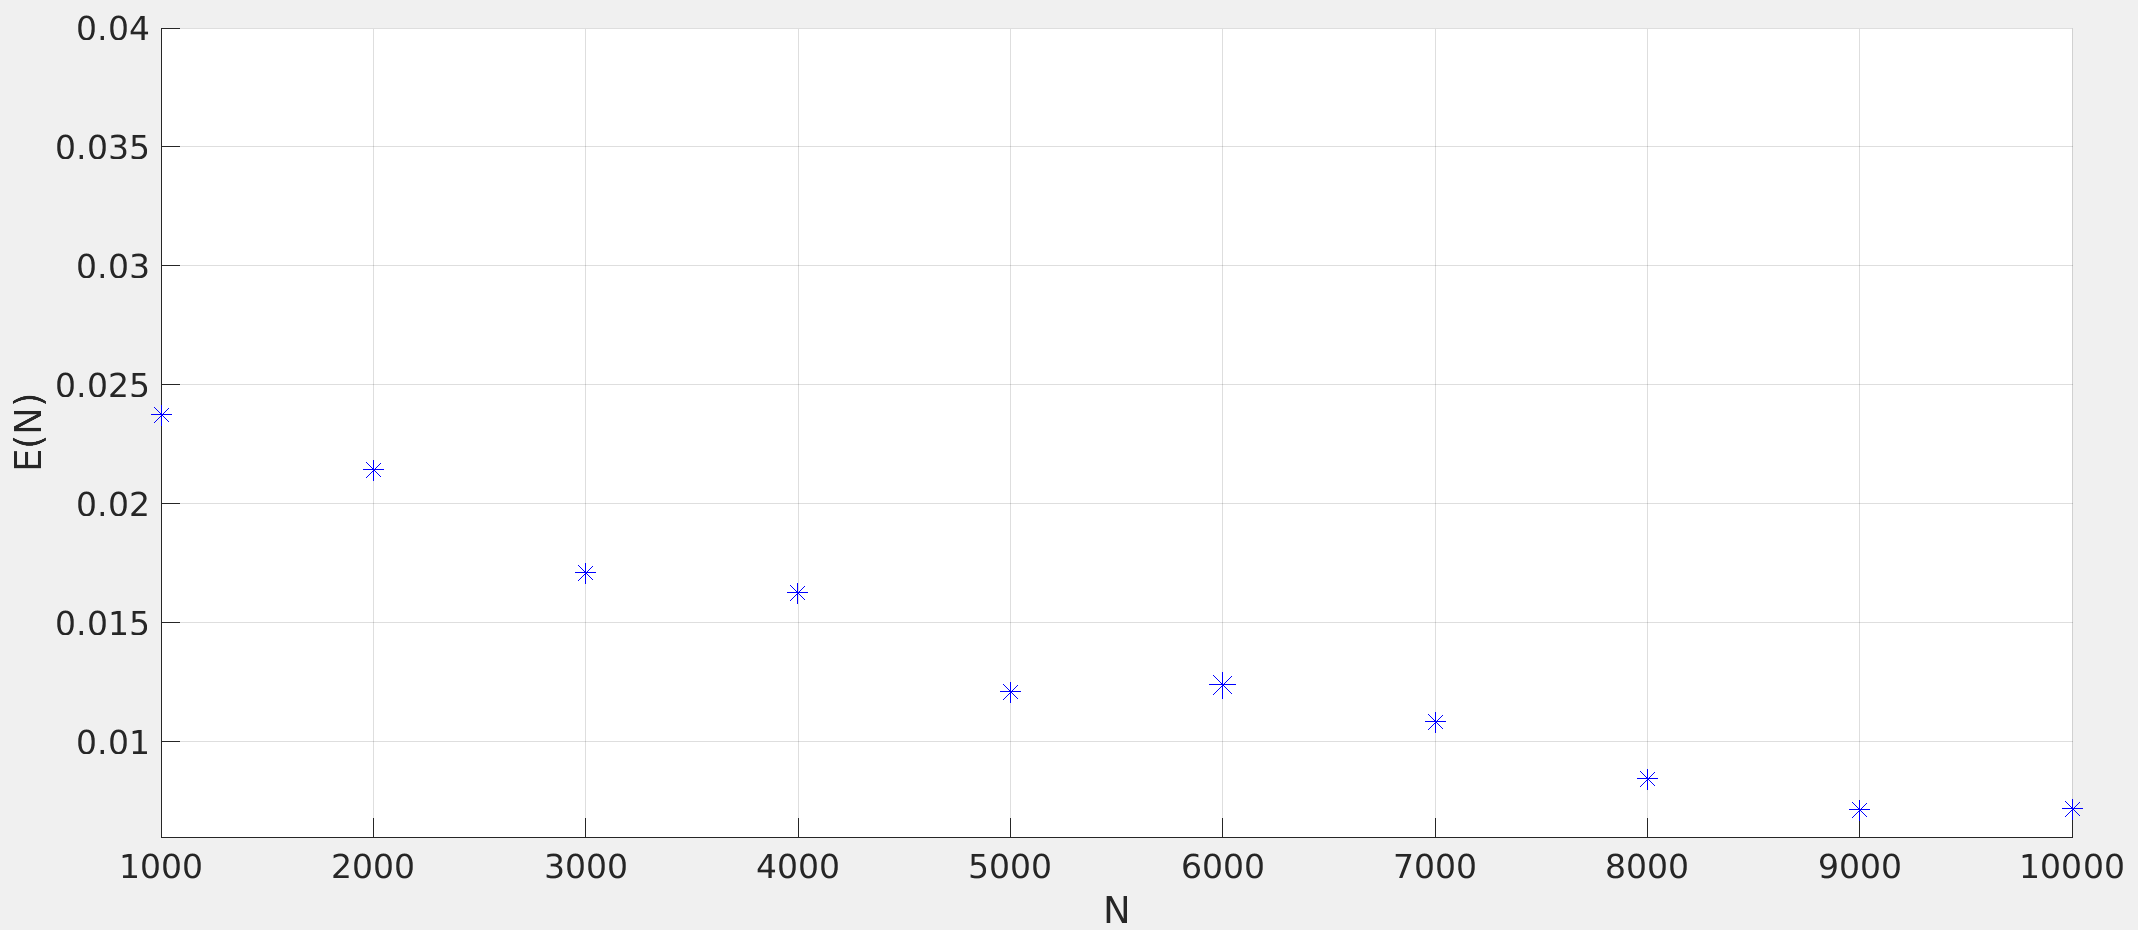
\includegraphics[width = \textwidth]{to2.png}
    \caption{Zależność średniego błędu estymatora od liczby pomiarów dla 5 wygenerowanych estymatorów}
    \label{blad_pomiaru1}
\end{figure}

\begin{figure}[H]
    \centering
    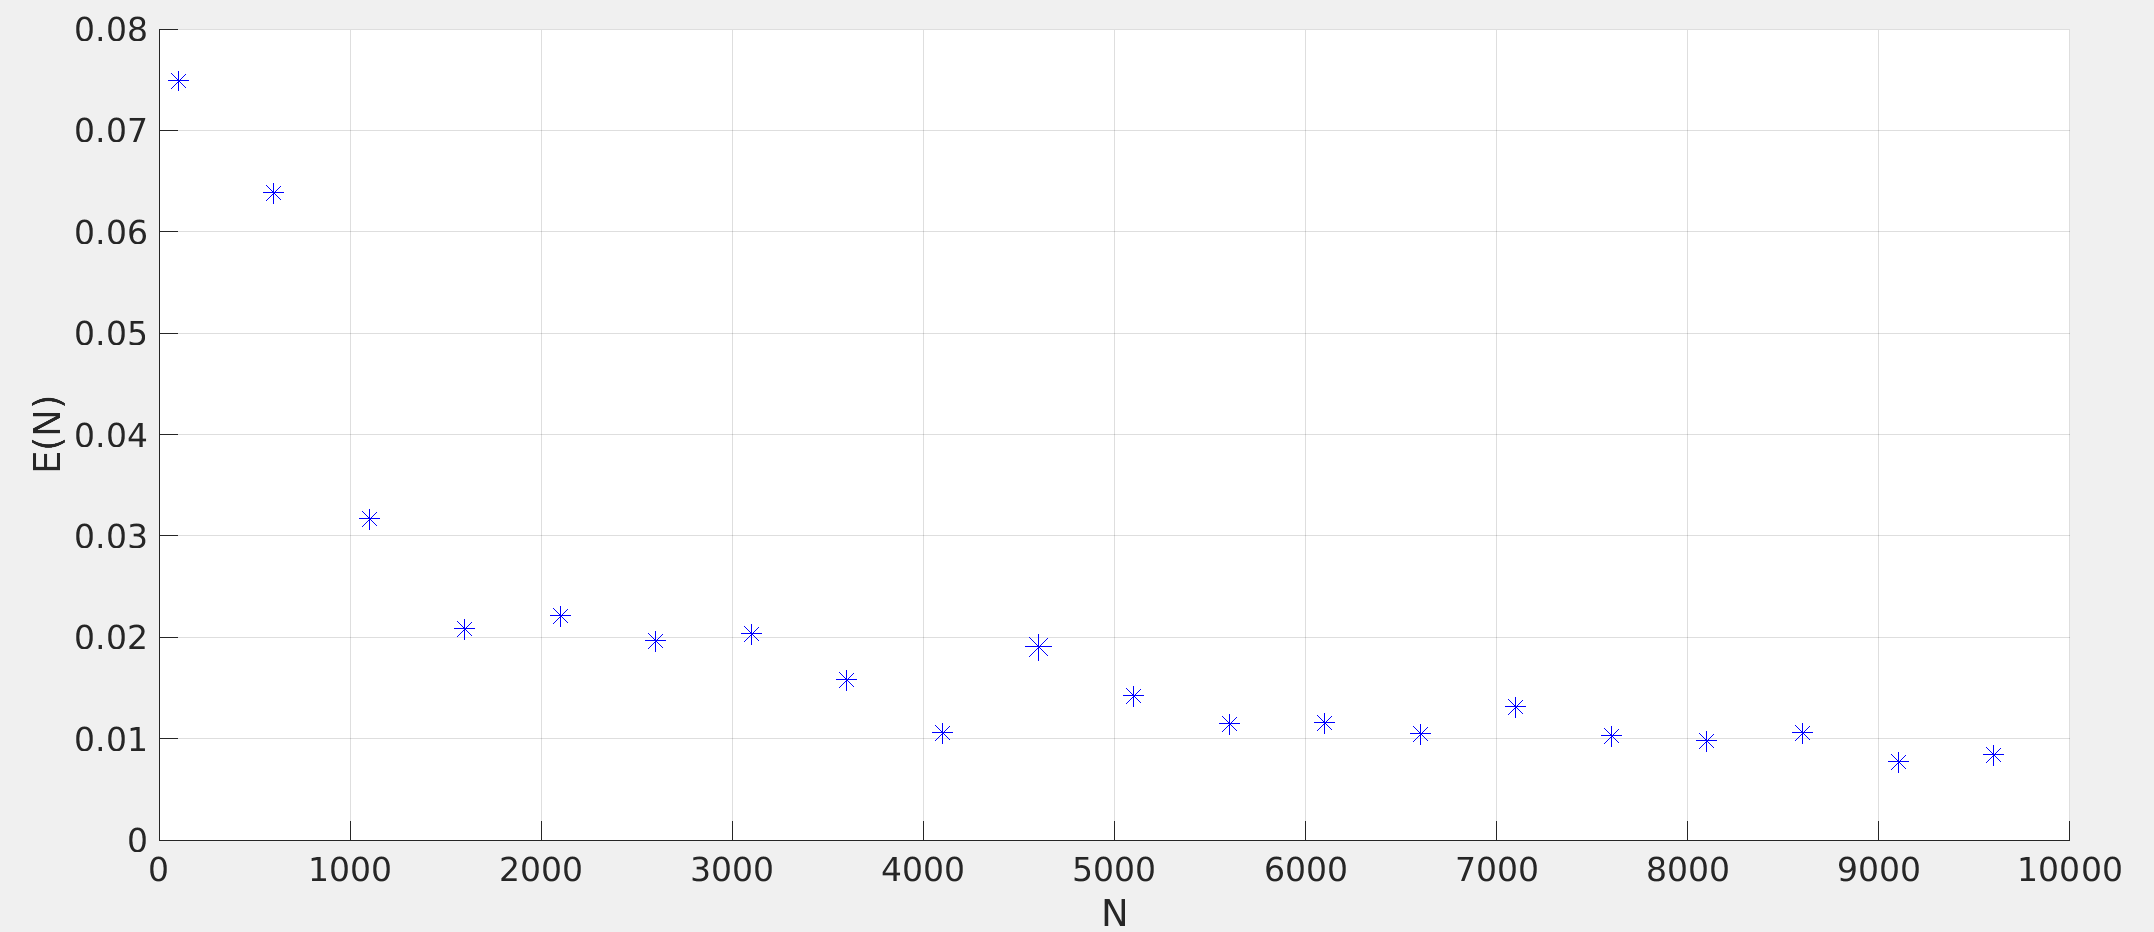
\includegraphics[width = \textwidth]{to3.png}
    \caption{Zależność średniego błędu estymatora od liczby pomiarów dla 10 wygenerowanych estymatorów}
    \label{blad_pomiaru2}
\end{figure}

\section{Podsumowanie i wnioski}
Po wykonaniu ćwiczenia sformułowano następujące wnioski:
\begin{itemize}
    \item Identyfikacja obiektu przebiegła poprawnie i pozwoliła na dokładne wyznaczenie parametrów opisujących badany obiekt.
    \item Wyznaczone wartości estymatora niewiele różniły się od rzeczywistych wartości, a po zaokrągleniu były z nimi identyczne.
    \item Średni błąd estymatora identyfikacji jest zależny od liczby pomiarów. Im więcej pomiarów, tym błąd estymatora dąży do 0. Na rys. \ref{blad_pomiaru2} dla 100 pomiarów błąd $E(N) \approx 0,075$, podczas gdy dla 10 000 pomiarów zmalał do wartości $E(N) \approx 0,01$.
    \item Funkcja błędu estymatora od liczby próbek przypomina funkcję eksponencjalną.
\end{itemize}

\end{document}